\documentclass[11pt]{article}
\usepackage[margin=0.8in]{geometry}
\usepackage{amsmath}
\usepackage[dvipsnames]{xcolor}
\usepackage{graphicx}
\usepackage{hyperref}
\usepackage{mathtools}
\usepackage{tikz,graphics,color,fullpage,float,epsf,caption,subcaption}
\DeclarePairedDelimiter{\floor}{\lfloor}{\rfloor}
% \usepackage[]{algorithm2e}
\usepackage{algorithm}
\usepackage{algorithmic}

\newcommand{\ggets}{\gets}



\title{CS3510-A: Design and Analysis of Algorithms, Spring 2021} 
\author{Homework-8}
\begin{document}
% \maketitle
\begin{center}
    
    \LARGE CS3510-A: Design and Analysis of Algorithms, Spring 2021 \\ \vspace{1em} 
    \large Homework-8 \\ \vspace{0.5em}
    March 7, 2021
\end{center}
\thispagestyle{empty}
\pagestyle{empty}

\noindent
\begin{center}
{\bf DUE DATE: Wednesday, March 17, 11:59pm}
\end{center}

\noindent
{\bf Note-1:} Your homework solutions should be electronically formatted as a single PDF document that you will upload on Gradescope. 
If you have to include some handwritten parts, please make sure that they are very clearly written and that you include them as high resolution images. \\

\noindent
{\bf Note-2:} Please think twice before you copy a solution from another student or resource (book, web site, etc). 
It is not worth the risk and embarrassment. \\

\noindent
{\bf Note-3:} You need to {\bf explain/justify} your answers. Do not expect full credit if you just state the correct answer. This includes their correctness and runtime.\\

\noindent
{\bf Note-4: You will get 2 extra points if you submit electronically typed solutions instead of hand-written.} 

\newpage
\section*{Problem-1 (30 points)}

Using Huffman encoding of n symbols with frequencies $f_1, f_2, ... f_n$, what is the length of the longest possible code-word? Additionally, what values of $f_1, f_2, ... f_n$ lead to this length? Please justify why these values of $f_i$ lead to the maximum possible length code-word.

\subsection*{Solution:}
The longest possible code word will be $n-1$.\\
The values of $f_1 .. f_n$ should be $f_x \gets \frac{1}{2^x}$.

\subsection*{Explanation:}
The Huffman algorithm for building an encoding tree makes a new merged node with the two nodes that have the lowest proabibilities.
By having probabilities that are each half of the next highest probability, the algorithm will merge each node with a subnode that includes all nodes with lower probabilities.
This will result in a tree that is the maximum possible depth and therefore have the longest possible code-word.

\newpage
\section*{Problem-2 (35 points)}

Suppose you’re consulting for a company that manufactures PC equipment and ships it to distributors all over the country. For each of the next $n$ weeks, they have a projected supply $s_i$ of equipment (measured in pounds), which has to be shipped by an air freight carrier.
\\
Each week’s supply can be carried by one of two air freight companies, A or B.
\begin{itemize}
    \item Company A charges a fixed rate $r$ per pound (so it costs $r*s_i$ to ship a week’s supply $s_i$).
    \item Company B makes contracts for a fixed amount $c$ per week, independent of the weight. However, contracts with company B must be made in blocks of four consecutive weeks at a time.
\end{itemize}
A schedule, for the PC company, is a choice of air freight company (A or B) for each of the n weeks, with the restriction that company B, whenever it is chosen, must be chosen for blocks of four contiguous weeks at a time. The cost of the schedule is the total amount paid to company A and B, according to the description above.
\\ \\
Example: Suppose $r = 1, c = 10$, and the sequence of values is 11,9,9,12,12,12,12,9,9,11. Then the optimal schedule would be to choose company A for the first three weeks, then company B for a block of four consecutive weeks, and then company A for the final three weeks.
\\ \\
Give a \textbf{polynomial-time} algorithm that takes a sequence of supply values $s_1, s_2, . . . , s_n$, which represent the supply for $n$ weeks, and returns a schedule of minimum cost. Note that you must not only return the \textbf{minimum cost} itself, but also the \textbf{schedule}.
\\ \\
Please provide your answer in four sections:
\begin{enumerate}
    \item Dynamic Programming Table: Must state the dimensions of the table, and explain what each element of this table represents.
    \item Recurrence Equation: Express mathematically each value in the table as a function of previous values in the table (do not forget to write down the equation(s) for the base case of the recursion).
    \item Pseudo-code: Construct your algorithm: takes $s_1, s_2, . . . , s_n$, $n, r, c$ as input and it should return the min cost as well as the schedule.
    \item Run-Time Analysis: Explain why your algorithm is polynomial time.
\end{enumerate}

\newpage
\subsection*{Solution:}
\subsection*{Dynamic Programming Table:}
The table for the solution of this problem will be one dimensional.
The table will essentially be an array with the optimal cost at each week for the given input data.

\subsection*{Recurrence Equation:}
For a week $i$ the optimal cost for that week can be calculated with: $min(rw_i + OPT_{i-1}, 4c + OPT_{i-4})$.
With a base case of $OPT_0 = 0$.

\subsection*{Pseudo-code:}
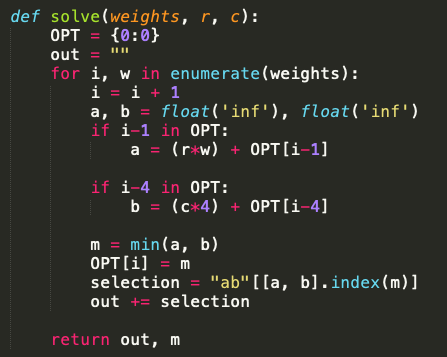
\includegraphics[scale=0.5]{two_code.png}

\subsection*{Run-Time:}
This algorithm will do $O(1)$ work for each of the $n$ weeks given.
Therefore, the overall runtime is $O(n)$.


\newpage
\section*{Problem-3 (35 points)}
Recall that in the basic Load Balancing Problem, we’re interested in placing jobs on machines so as to minimize the makespan— the maximum load on any one machine. In a number of applications, it is natural to consider cases in which you have access to machines with different amounts of processing power, so that a given job may complete more quickly on one of your machines than on another. The question then becomes: How should you allocate jobs to machines in these more heterogeneous systems?
\\ \\
Here’s a basic model that exposes these issues. Suppose you have a system that consists of $m$ slow machines and $k$ fast machines. The fast machines can perform twice as much work per unit time as the slow machines. Now you’re given a set of \textit{n} jobs; job $i$ takes time $\mathit{t_i}$ to process on a slow machine and time $\mathit{(1/2)t_i}$ to process on a fast machine. You want to assign each job to a machine; as before, the goal is to minimize the makespan -- that is the maximum, over all machines, of the total processing time of jobs assigned to that machine.
\\ \\
Describe a \textbf{polynomial-time algorithm} that produces an assignment of jobs to machines with a makespan that is at most three times the optimum. Your solution should be of the form:
\begin{itemize}
    \item Algorithm and runtime: Briefly describe how you will assign tasks to machines -- and explain why your algorithm can run in poly-time. (This part can be done with 1-2 sentences only!)
    \item Proof of Upper Bound: Show why your greedy solution can have a makespan that is at most 3 times the optimal solution's makespan.
\end{itemize}

\newpage
\subsection*{Solution:}
\begin{algorithm}
    \caption{Sorted-Balance for Heterogeneous setting}
    \begin{algorithmic}[1]
        \STATE Start with no jobs assigned
        \STATE $T_i = 0$ and $A(i)=\emptyset$ for all machines $M_i$
        \STATE Sort jobs in decreasing order of processing times $t_j$
        \STATE Assume that $t_1 \geq t_2 \geq ... \geq t_n$

        \FOR{$j = 1, ..., n$}
            \STATE $F_i \gets $ fast machine with the minimum $min_k T_k$
            \STATE $S_i \gets $ slow machine with the minimum $min_k T_k$
            \IF{$T_S + t_j > T_F + \frac{t_j}{2}$}
                \STATE $M_i \gets F_i$
            \ELSE
                \STATE $M_i \gets S_i$
            \ENDIF

            \STATE Assign job to $M_i$
            \STATE Set $A(i) \gets A(i) \cup {j}$
            \IF{$M_i$ is a fast machine}
                \STATE Set $T_i \gets T_i + \frac{t_j}{2}$
            \ELSE
                \STATE Set $T_i \gets T_i + t_j$
            \ENDIF
        \ENDFOR
    \end{algorithmic}
\end{algorithm}

\subsection*{Explanation:}
This algorithm is the same as the one from section 11.1 of the book.
However this algorithm accounts for faster machines being able to process double the amount of work
by adding half of the job load to the appropriate $T$ when a fast machine is chosen.

\subsection*{Runtime:}
\begin{itemize}
\itemsep0em
\item Sorting the jobs in decreasing order can be done in $O(nlogn)$
\item For $n$ jobs:\\
    \begin{itemize}
        \itemsep0em 
        \vspace{-0.6cm} \item The machine with minimum job load can be found and removed with a Fibonnaci heap in $O(logm)$ or $O(logk)$
        \item The machine job load is then updated with the current job added as a new point in a Fibonnaci heap in $O(1)$.
    \end{itemize}
\end{itemize}
These runtimes reduce down to $O(n)$ which is polynomial time.

\subsection*{Proof of Upper Bound:}
Where $t_j$ is the load of the largest job.
If the largest job were placed on the fastest machine, then $t_j \leq 2T^*$ (where $T^*$ is the makespan of the optimal solution).\\
Where $T_i$ is the makespan of the machine that has recieved job $j$, $T_i - t_j \leq T^*$
(the load on the machine before it recieves job $j$ will be less than the optimal makespan).\\
This can be rewritten as: $T_i - 2T^* \leq T^*$. And then reduced to: $T_i \leq 3T^*$.\\
Thus, the makespan of this greedy solution is at most 3 times the optimal solution's makespan.


\end{document}